%=========================================================================
%  Conference-format manuscript (IEEEtran, two-column).
%
%  Compiles as-is on Overleaf: IEEEtran.cls ships with every TeX Live /
%  Overleaf install; the three figures are produced by
%  scripts/reproduce_results.py into ./figs/.
%
%  Every numeric claim in this file is emitted by that script (Granger/FDR
%  by src/models/causal_validation.py, truncation by --tokens). Do not edit
%  a number here by hand -- change the analysis and re-run, so the paper and
%  the code cannot drift apart.
%=========================================================================
\documentclass[conference]{IEEEtran}
\IEEEoverridecommandlockouts

\usepackage{cite}
\usepackage{amsmath,amssymb,amsfonts}
\usepackage{graphicx}
\usepackage{booktabs}
\usepackage{multirow}
\usepackage{url}
\usepackage[hidelinks]{hyperref}

\begin{document}

\title{Does Political Communication Predict Indian Equity Returns?\\
\large A Null Result, and How Evaluation Design Manufactures Accuracy}

\author{
\IEEEauthorblockN{Dirshak Deepak Patro}
\IEEEauthorblockA{\textit{Department of Information Technology} \\
\textit{Somaiya Vidyavihar University}\\
Mumbai, India \\
dirshak.p@somaiya.edu}
\and
\IEEEauthorblockN{Disha Kataria}
\IEEEauthorblockA{\textit{Department of Information Technology} \\
\textit{Somaiya Vidyavihar University}\\
Mumbai, India \\
disha.kataria@somaiya.edu}
}

\maketitle

\begin{abstract}
Political leadership communication is widely assumed to move financial markets, and a growing literature reports directional accuracies of 74--87\% from NLP pipelines built on such text. We construct one of these pipelines end to end and test the assumption directly. Our corpus comprises 1{,}288 leadership communications spanning May 2016 to August 2026 --- Mann ki Baat broadcasts, European Central Bank speeches, and U.S. Federal Reserve communications --- aligned to daily prices for 16 Indian and global instruments, yielding 16{,}832 analysable event observations. We evaluate under a cross-sectional design whose baseline is pinned at exactly 50\% by construction, with expanding-window walk-forward refits and standard errors clustered by event date. Rhetoric features score 49.99\% ($z=-0.63$); a horizon sweep from 1 to 252 trading days finds rhetoric-only accuracy confined to 49.88--50.02\% at every lag, ruling out delayed transmission. Under the absolute-direction framing, fitted models underperform a naive always-up rule by 5.86 percentage points ($z=-6.00$). Granger tests across ten topics yield zero discoveries surviving Benjamini--Hochberg correction, against a procedure whose null expectation is 2.26 nominal hits. As a positive control we show the same pipeline predicts realized-volatility direction at 68.67\% ($+17.07$pp over baseline, $z=+23.75$) --- but rhetoric contributes nothing there either ($-0.62$pp, $p=0.17$), and neither does India VIX. Finally we quantify how evaluation design manufactures accuracy: at a 252-day horizon our model reports 75.28\%, a figure that would headline a paper, while being 3.58pp \emph{worse} than a constant rule. We release the pipeline and evaluation harness.
\end{abstract}

\begin{IEEEkeywords}
market efficiency, political communication, null result, topic modeling, FinBERT, Granger causality, false discovery rate, backtest overfitting, walk-forward validation, realized volatility, Indian equity markets
\end{IEEEkeywords}

%=========================================================================
\section{Introduction}
%=========================================================================
Classical theory holds that asset prices reflect all publicly available information \cite{fama1970}, yet an extensive literature documents apparent deviations around political and policy events. Leadership communication --- speeches, press conferences, and broadcast addresses such as \textit{Mann ki Baat} --- is a natural candidate for a high-density information channel shaping expectations, sector rotation, and risk appetite. The Indian equity market is an attractive setting, subject both to domestic policy communication and to monetary signals from the Federal Reserve and ECB that propagate through capital-flow and currency channels.

A reasonable hypothesis follows: a pipeline that ingests this communication, resolves its topical content, scores its sentiment, and aligns it to market data should extract measurable directional predictability. We built that pipeline and tested that hypothesis. It does not survive.

We report the null as the primary finding for three reasons. First, it is established under a design whose baseline is exactly 50\%, so it cannot be attributed to equity drift, and it holds across every forecast horizon from one day to one year. Second, the accuracies commonly reported in this area --- 74\% \cite{jain2023}, 87\% \cite{biswal2022}, $R^2=0.9866$ \cite{bhandari2025} --- are difficult to reconcile with market efficiency, and we reproduce figures in exactly that band on our own data using choices that add no predictive content. Third, a null accompanied by a reproducible harness is more useful than an unreplicable positive.

To establish that the null reflects the data rather than a weak pipeline, we include a positive control: the same features and protocol predict realized-volatility direction at 68.67\%, $+17.07$ percentage points over baseline at $z=+23.75$. The machinery works. Rhetoric simply carries no directional information.

The distinction we press throughout is between \textit{accuracy} and \textit{skill}. An accuracy figure is uninterpretable without three companions: the baseline a trivial rule achieves on the same test window, the coverage over which it is computed, and the clustering used for inference. Omit any one and a null becomes indistinguishable from a strong result.

\textbf{Contributions.}
\begin{enumerate}
\item A reproducible multi-source pipeline over 1{,}288 documents and 16 instruments (2016--2026).
\item A null result for return direction, robust across two targets, three model classes, and eight forecast horizons, with an ablation localizing all marginal effect to price momentum rather than rhetoric.
\item A positive control on realized volatility (68.67\%, $z=+23.75$) demonstrating the null is a property of the signal, not the method --- and a second null showing rhetoric adds nothing there either.
\item A quantified account of how four routine evaluation choices manufacture 72.7--100\% accuracy on this data, including a 252-day configuration reporting 75.28\% while underperforming a constant rule.
\end{enumerate}

%=========================================================================
\section{Related Work}
%=========================================================================
\textbf{Price-based deep learning.} Bhandari et al.\ \cite{bhandari2025} combine a GRU over prices with FinBERT and BERTopic news features, reporting $R^2=0.9866$ --- a level more consistent with a highly autocorrelated target (price level) than with directional skill. Khadke et al.\ \cite{khadke2023} report $R^2$ of 0.922 for CNN versus 0.88 for LSTM; Kumar et al.\ \cite{kumar2024} report 2.36\% error for LSTM. These establish architectural baselines but do not report what a persistence or always-up rule achieves on the same series. Nazari et al.\ \cite{nazari2025} provide the essential counterweight, warning that such models often fail to beat buy-and-hold; our Table~\ref{tab:horizon} corroborates this at every horizon. Chen et al.\ \cite{chen2024} model asymmetric lead-lag structure across stocks, motivating our instrument-identity and cross-sectional relative features.

\textbf{Financial NLP.} Araci \cite{araci2019} introduced FinBERT by further-pretraining on financial corpora; Paul et al.\ \cite{paul2024} report 89.6\% classification accuracy. Loughran and McDonald \cite{loughran2011} established that general-purpose sentiment dictionaries systematically misclassify financial language. Rambola et al.\ \cite{rambola2021} link public-figure sentiment to abnormal returns; Jain et al.\ \cite{jain2023} report 74\% from headline embeddings; Biswal et al.\ \cite{biswal2022} report 87\% via Grey Relational Analysis. The recurrence of the 74--87\% band across heterogeneous methods and markets is the observation motivating Section~\ref{sec:inflate}.

\textbf{Topic models and event studies.} Seng and Lim \cite{seng2023} show BERTopic features improve downstream error metrics; Buehlmaier and Whited \cite{buehlmaier2018} apply LDA to 70{,}000 8-K filings; Mishev et al.\ \cite{mishev2022} disentangle co-occurring announcement topics. For the Indian setting, Srivastava and Mitra \cite{srivastava2019} find significant abnormal returns around the Pulwama--Balakot crisis persisting roughly 11 days. A discrete unanticipated geopolitical shock and a decade of scheduled monthly broadcasts are different objects; our results suggest the latter does not inherit the predictability of the former.

\textbf{Multiple testing and overfitting.} White \cite{white2000} introduced the reality-check bootstrap for data snooping. Harvey et al.\ \cite{harvey2016} argue most published cross-sectional predictors are false discoveries under proper multiplicity accounting. Bailey et al.\ \cite{bailey2014} formalize backtest overfitting. Benjamini and Hochberg \cite{benjamini1995} supply the FDR procedure we apply. Gu et al.\ \cite{gu2020} provide the evaluation template we follow. This toolkit is standard in asset pricing and comparatively underused in the political-communication literature.

%=========================================================================
\section{Data and Pipeline}
%=========================================================================
\subsection{Corpus}
Table~\ref{tab:corpus} summarizes the data. Of 1{,}288 documents, 1{,}071 carry a parseable date; after joining sentiment and topic features and requiring complete trailing market windows, 1{,}052 documents yield 16{,}832 (document, instrument) observations across 798 event dates.

\begin{table}[t]
\caption{Assembled corpus and derived records.}
\label{tab:corpus}
\centering
\small
\begin{tabular}{lr}
\toprule
\textbf{Quantity} & \textbf{Count} \\
\midrule
Documents, total & 1{,}288 \\
\quad U.S. Federal Reserve & 746 \\
\quad European Central Bank & 472 \\
\quad Mann ki Baat & 70 \\
\quad with parseable date & 1{,}071 \\
Date span & 2016-05-19 -- 2026-08-05 \\
Market instruments & 16 \\
Daily observations (with returns) & 46{,}480 \\
Event observations & 17{,}104 \\
\quad entering analysis & 16{,}832 \\
Sentiment scores & 1{,}287 \\
Topic assignments (pooled model) & 12{,}870 \\
HMM regime classifications & 3{,}053 \\
India VIX observations & 2{,}959 \\
\bottomrule
\end{tabular}
\end{table}

Mann ki Baat coverage is 70 of 125 numbered episodes; episodes 22--75 and 102 are absent from our source and reported as missing rather than imputed. The pooled corpus is consequently 94.6\% central-bank text, which we treat as a limitation rather than a design choice.

\subsection{Text Processing}
Documents are lowercased and stripped of URLs and non-alphanumeric content, then processed with spaCy. A part-of-speech filter retains nouns, proper nouns, verbs, and adjectives, which are lemmatized; short tokens, stopwords, and a domain stopword list of rhetorical formulae are removed. A Devanagari detector routes Hindi-dominant documents to an indic-nlp path; in the assembled corpus all Mann ki Baat transcripts are English, so this path is exercised only incidentally.

Topics come from TF-IDF followed by Non-negative Matrix Factorization with $K=10$, factorizing the term-document matrix $\mathbf{M}$ into non-negative $\mathbf{W},\mathbf{H}$ with $\mathbf{M}\approx\mathbf{WH}$. We initially implemented an LDA/NMF/BERTopic ensemble with coherence-weighted averaging and removed it: on a corpus of order $10^3$ documents the UMAP--HDBSCAN stage produced unstable clusters with large noise assignments, and ensemble coherence did not exceed NMF alone. We record this negative architectural result because it runs against the prevailing assumption that ensembling helps.

FinBERT assigns each document probabilities over \{positive, negative, neutral\}; we retain all three plus a compound score. Its 512-token limit truncates every document, and the severity is easy to understate. Measured with the model's own tokenizer over 40 documents per source, the median Mann ki Baat transcript is 4{,}804 tokens, so FinBERT observes \textbf{10.7\%} of it; the figures are 17.6\% for ECB and 13.8\% for Fed. Our sentiment features describe each document's opening passage, not the document.

\subsection{Market Features}
A three-state Gaussian HMM fitted to index log-returns by Baum--Welch assigns each trading day a latent regime. Asset-specific baseline normalization expresses price as a trailing 252-day $z$-score. For each (document, instrument) pair we compute forward cumulative returns $r^{(n)}=\prod_{k=1}^{n}(1+r_{t+k})-1$ and forward realized volatility $\sigma^{(n)}=\mathrm{sd}(r_{t+1..t+n})$.

We target raw $r^{(n)}$ rather than the pipeline's abnormal-return field, which subtracts a \textit{full-sample} mean and therefore embeds post-event information. The magnitude effect is modest, but the analysis of interest is a sign test and the subtraction flips the sign of 4.6\% of events --- a caution that generalizes: a constant per-instrument offset is harmless for ranking and consequential for direction.

%=========================================================================
\section{Evaluation Protocol}
\label{sec:protocol}
%=========================================================================
\textbf{Targets.} The \textit{absolute} target is $y=\mathbf{1}[r^{(n)}>0]$; its baseline is the majority class, which exceeds 50\% because equity returns drift upward. The \textit{cross-sectional} target is
\begin{equation}
y_{ij}=\mathbf{1}\!\left[r^{(n)}_{ij}>\operatorname{median}_j\!\left(r^{(n)}_{ij}\right)\right],
\label{eq:xs}
\end{equation}
asking whether instrument $j$ outperforms the median instrument following document $i$. Ties are dropped. This baseline is \textit{exactly} 50\% by construction, removing drift as a confound; our central claim rests on it. A third target, \textit{volatility direction} $\mathbf{1}[\sigma^{(n)}_{\text{fwd}}>\sigma^{(n)}_{\text{trailing}}]$, serves as a positive control.

\textbf{Features (196).} All computed strictly from pre-$t_i$ information: 5 sentiment, 10 topic probabilities, 160 topic$\times$instrument interactions, 16 instrument indicators, and 5 market controls (relative momentum over 5/10/20/60 observations and relative 20-day realized volatility), demeaned within each event as a relative target requires. The interactions encode the hypothesis under test.

\textbf{Validation.} Expanding-window walk-forward with five folds: fitted on all observations up to a fold boundary, predicting only the subsequent block, so no test observation informs any fit that predicts it.

\textbf{Inference.} Each document contributes one observation per instrument and these are not independent. Hit indicators are averaged within event date and standard errors computed across the 484 resulting cluster means.

%=========================================================================
\section{Results}
%=========================================================================
\subsection{Return Direction}
Table~\ref{tab:main} reports the central result. The strongest specification, gradient boosting, reaches 51.71\% against a 50\% baseline ($z=+2.90$) --- nominally significant across three specifications tested.

The ablation settles its interpretation. Restricting to rhetoric features alone --- sentiment and topic probabilities, the quantities this paper is about --- yields 49.99\% ($z=-0.63$), indistinguishable from chance, as do the topic$\times$instrument interactions in isolation (50.04\%). Market controls alone yield 50.63\%. The marginal edge is attributable to price momentum, not to leadership communication. On the hypothesis under test, the result is a clean null.

\begin{table}[t]
\caption{Out-of-sample accuracy, cross-sectional 5-day target. Baseline exactly 50.0\%. $n=10{,}099$ predictions across 484 event-date clusters; SEs clustered by date.}
\label{tab:main}
\centering
\small
\begin{tabular}{lccc}
\toprule
\textbf{Specification} & \textbf{Hit} & \textbf{SE} & \textbf{$z$} \\
\midrule
\multicolumn{4}{l}{\textit{Full feature set (196)}} \\
\quad Logistic ($C=0.05$) & 51.16\% & 0.68pp & $+1.70$ \\
\quad Logistic ($C=1$) & 51.12\% & 0.68pp & $+1.65$ \\
\quad Gradient boosting & 51.71\% & 0.59pp & $+2.90$ \\
\midrule
\multicolumn{4}{l}{\textit{Feature-group ablation (logistic, $C=1$)}} \\
\quad \textbf{Rhetoric only (sentiment + topics)} & \textbf{49.99\%} & --- & $\mathbf{-0.63}$ \\
\quad Topic $\times$ instrument only & 50.04\% & --- & $+0.06$ \\
\quad Market controls only & 50.63\% & --- & $+0.92$ \\
\bottomrule
\end{tabular}
\end{table}

Under the absolute-direction target the picture is worse: an always-up rule achieves 56.46\%, gradient boosting 50.60\%, an edge of $-5.86$pp ($z=-6.00$). The fitted model is significantly worse than ignoring the data.

\subsection{Is There a Transmission Lag?}
A natural defence of the null is that rhetoric acts slowly, so a five-day window is simply too short. Table~\ref{tab:horizon} tests this directly across eight horizons.

\begin{table}[t]
\caption{Horizon sweep. ``Raw'' is absolute-target accuracy --- the figure a horizon-tuned claim would report; ``base'' is the always-up rule on the same window. Rhetoric-only uses the cross-sectional target (baseline exactly 50\%).}
\label{tab:horizon}
\centering
\small
\begin{tabular}{rccrcr}
\toprule
\textbf{$h$} & \textbf{Raw} & \textbf{Base} & \textbf{Edge} & \textbf{Rhet.\ only} & \textbf{$z$} \\
\midrule
1 & 52.20\% & 52.33\% & $-0.14$ & 50.02\% & $+0.54$ \\
5 & 55.12\% & 56.41\% & $-1.29$ & 49.99\% & $-0.63$ \\
10 & 57.46\% & 59.25\% & $-1.80$ & 50.00\% & $+0.16$ \\
20 & 58.30\% & 60.21\% & $-1.91$ & 49.98\% & $-0.76$ \\
30 & 59.00\% & 60.85\% & $-1.85$ & 49.99\% & $-0.33$ \\
60 & 62.39\% & 64.41\% & $-2.02$ & 49.94\% & $-1.26$ \\
120 & 64.25\% & 68.44\% & $-4.19$ & 49.91\% & $-0.78$ \\
\textbf{252} & \textbf{75.28\%} & \textbf{78.85\%} & $\mathbf{-3.58}$ & 49.88\% & $-1.74$ \\
\bottomrule
\end{tabular}
\end{table}

Two findings. First, rhetoric-only accuracy is confined to 49.88--50.02\% at \textit{every} horizon; there is no lag at which leadership communication predicts relative returns, so the slow-transmission defence fails on its own terms.

Second, and central to Section~\ref{sec:inflate}: raw accuracy rises monotonically with horizon, reaching 75.28\% at one year --- a figure that would comfortably headline a paper. On the same window a constant ``up'' call scores 78.85\%. The model is 3.58pp \textit{worse} than doing nothing, at $z=-3.91$. Fig.~\ref{fig:horizon} shows the two curves; the visible gap between them is negative throughout.

\begin{figure}[t]
\centering
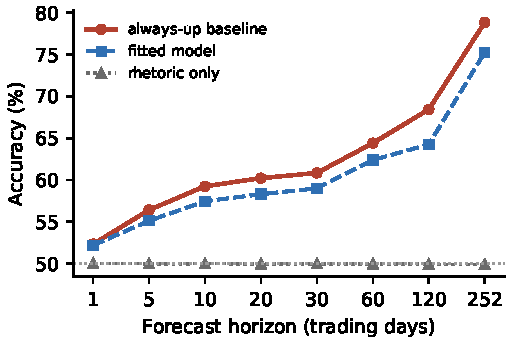
\includegraphics[width=\columnwidth]{figs/fig_horizon.pdf}
\caption{Accuracy by forecast horizon. The fitted model (squares) tracks below the always-up baseline (circles) at every horizon, while rhetoric-only accuracy (triangles) stays pinned at 50\%. Reporting the model curve alone would suggest steadily improving performance.}
\label{fig:horizon}
\end{figure}

\subsection{Positive Control: Volatility}
If the pipeline were simply weak, it would fail everywhere. Table~\ref{tab:vol} shows it does not: the same features and protocol predict realized-volatility direction far above baseline.

\begin{table}[t]
\caption{Volatility direction (will realized volatility rise or fall?). The pipeline works --- but rhetoric contributes nothing, and neither does India VIX. Increments are paired over date clusters.}
\label{tab:vol}
\centering
\small
\begin{tabular}{llcc}
\toprule
\textbf{$h$} & \textbf{Features} & \textbf{Hit} & \textbf{Edge vs base} \\
\midrule
\multirow{1}{*}{10d}
 & Market only & 68.67\% & $+17.07$pp ($z=+23.75$) \\
 & Rhetoric only & 50.82\% & $-0.79$pp \\
 & \textit{rhetoric increment} & \multicolumn{2}{l}{$-0.62$pp, $p=0.17$} \\
\midrule
\multirow{1}{*}{20d}
 & Market only & 66.04\% & $+13.39$pp ($z=+20.48$) \\
 & Rhetoric only & 50.40\% & $-2.26$pp \\
 & \textit{rhetoric increment} & \multicolumn{2}{l}{$+0.61$pp, $p=0.19$} \\
\midrule
\multirow{1}{*}{30d}
 & Market only & 65.93\% & $+12.85$pp ($z=+17.96$) \\
 & Rhetoric only & 49.77\% & $-3.31$pp \\
 & \textit{rhetoric increment} & \multicolumn{2}{l}{$-0.11$pp, $p=0.81$} \\
\bottomrule
\end{tabular}
\end{table}

Volatility direction is predicted at 68.67\% against a 51.60\% baseline, an edge of $+17.07$pp at $z=+23.75$. This is volatility clustering, a well-established property of return series, and it establishes that our walk-forward harness detects real structure when real structure exists.

Rhetoric adds nothing to it. Incremental contributions across the three horizons are $-0.62$, $+0.61$, and $-0.11$ percentage points ($p=0.17$, $0.19$, $0.81$) --- inconsistent in sign and individually insignificant. India VIX, a direct forward-looking volatility measure previously unused in the pipeline, adds $+0.07$, $-0.04$, and $+0.33$pp ($p=0.90$, $0.94$, $0.55$). The second-moment channel, which we had considered the most plausible remaining route for a communication effect, is also null.

\begin{figure}[t]
\centering
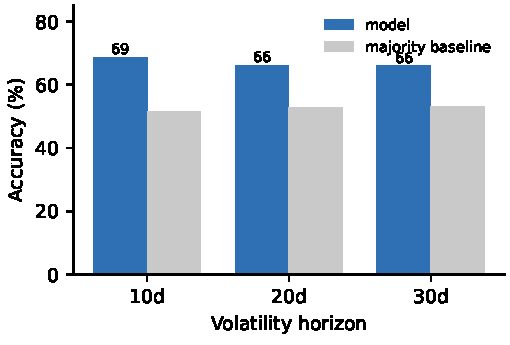
\includegraphics[width=\columnwidth]{figs/fig_volatility.pdf}
\caption{Volatility direction: model versus majority baseline. The large, highly significant edge here is the positive control --- the same protocol that returns 50\% on rhetoric returns 66--69\% when genuine structure is present.}
\label{fig:vol}
\end{figure}

\subsection{Granger Causality with FDR Control}
Table~\ref{tab:granger} tests whether topic intensity Granger-causes market returns, taking the minimum F-test $p$-value over lags 1--5.

\begin{table}[t]
\caption{Granger causality, topic intensity $\rightarrow$ returns. Raw $p$ is the minimum over lags 1--5; $q$ is the Benjamini--Hochberg adjustment across ten topics.}
\label{tab:granger}
\centering
\small
\begin{tabular}{lcc}
\toprule
\textbf{Topic} & \textbf{Raw $p$} & \textbf{BH $q$} \\
\midrule
Respondent, Quintile, SPF & 0.0100 & 0.100 \\
Financial Stability \& Markets & 0.0539 & 0.183 \\
Labor, Inflation, Percent & 0.0550 & 0.183 \\
ECB, European, Medium Query & 0.1622 & 0.406 \\
Payment, Digital, Stablecoin & 0.3096 & 0.521 \\
Term Condition, Net, Survey Round & 0.3124 & 0.521 \\
Village, Life, Youth & 0.4026 & 0.575 \\
Monetary Policy \& Inflation & 0.4604 & 0.576 \\
National Unity \& Commemoration & 0.6233 & 0.693 \\
Euro Area, Euro, ECB & 0.7501 & 0.750 \\
\midrule
\multicolumn{3}{l}{\textbf{Discoveries at $q<0.05$: 0 of 10}} \\
\bottomrule
\end{tabular}
\end{table}

No topic survives correction. More instructive: taking a minimum across five lags is itself a selection procedure. Under the null, $P(\min_{1..5}p<0.05)=1-0.95^5=0.226$, so across ten topics the expected number of nominal hits is 2.26. We observe one. The raw count is \textit{below} chance expectation, and an uncorrected reading --- which would report one significant topic --- inverts the actual inference. The sole nominal hit loads on \textit{respondent}, \textit{quintile}, and \textit{SPF}: vocabulary from the ECB Survey of Professional Forecasters, describing survey instrumentation rather than economic rhetoric.

\subsection{How Evaluation Design Manufactures Accuracy}
\label{sec:inflate}
Table~\ref{tab:inflate} applies four routine choices to this same data. Each yields a figure in the band this literature reports; none adds predictive skill.

\begin{table}[t]
\caption{Accuracy obtainable on this dataset without predictive skill.}
\label{tab:inflate}
\centering
\small
\begin{tabular}{p{2.9cm}cp{3.4cm}}
\toprule
\textbf{Choice} & \textbf{Reported} & \textbf{What it is} \\
\midrule
Horizon $\rightarrow$ 252 days & 74.5\% & Always-up baseline is \textit{also} 74.5\% \\
Random forest, no train/test split & 100.0\% & Memorization of 16{,}832 rows \\
Post-event variable among features & 72.7\% & Target algebraically inside features \\
Top 1\% most-confident only & 78.0\% \textit{or} 50.0\% & $n=50$; flips with target choice \\
\bottomrule
\end{tabular}
\end{table}

The horizon effect deserves emphasis as the least obviously improper, and Table~\ref{tab:horizon} shows why: a researcher who tunes the window to maximize reported accuracy lands at 252 days and 75.28\%, which is both an attractive number and 3.58pp worse than a constant rule.

The selective-reporting case is subtler, since restricting to high-confidence predictions is defensible as selective prediction. The defence fails on two grounds. First, the coverage curve (Fig.~\ref{fig:coverage}) is non-monotonic --- 51.2\%, 50.6\%, 49.3\%, 49.8\%, 50.7\%, 51.7\% as coverage falls from 100\% to 2\% --- whereas genuine confidence calibration produces a monotone increase. Second, and decisively, the same top-1\% procedure with identical features and split yields 78.0\% under the absolute target and 50.0\% under the cross-sectional target. A statistic whose value depends on the target definition at $n=50$ is noise.

\begin{figure}[t]
\centering
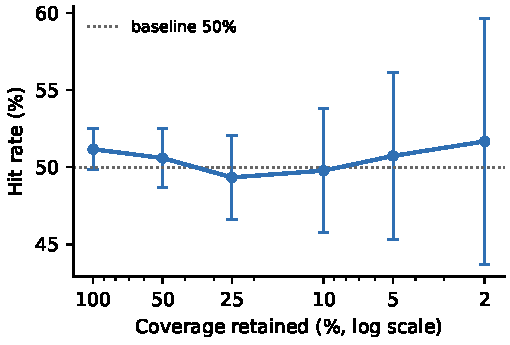
\includegraphics[width=\columnwidth]{figs/fig_coverage.pdf}
\caption{Hit rate against retained coverage, with 95\% intervals from date-clustered standard errors. Calibrated confidence would rise monotonically as coverage falls; this curve wanders within its intervals.}
\label{fig:coverage}
\end{figure}

\subsection{Pseudo-Replication}
Each document generates one record per instrument, and the instruments co-move strongly: mean pairwise correlation of event-window returns is $\rho=0.414$ across $k=16$ instruments. The design effect is
\begin{equation}
\mathrm{deff}=1+(k-1)\rho=1+15(0.414)=7.2,
\label{eq:deff}
\end{equation}
so an apparent 10{,}099 records carry the information of roughly 1{,}400, and unclustered standard errors are understated by $\sqrt{7.2}=2.68\times$. Reported significance that does not state its clustering scheme is uninterpretable in this setting.

%=========================================================================
\section{Discussion}
%=========================================================================
The most economical explanation is the standard one. Mann ki Baat is a pre-announced, nationally broadcast monthly address; ECB and Fed communications are scheduled and intensely scrutinized. Any information content reaches all participants simultaneously at zero cost, and weak-form efficiency \cite{fama1970} predicts incorporation faster than a daily-resolution pipeline can act on.

Three pieces of evidence make this hard to attribute to a weak implementation. The ablation shows rhetoric at exactly chance while momentum controls carry the entire marginal effect. The horizon sweep shows the same at every lag from one day to one year, closing off delayed transmission. And the volatility control shows the identical harness detecting a $+17$pp effect where genuine structure exists. A pipeline that finds volatility clustering at $z=+23.75$ and rhetoric at $z=-0.63$ is not failing to look.

This does not establish that leadership communication is irrelevant to markets. It establishes something narrower: at daily resolution, over a decade of routine communications, using topic distributions and document-level sentiment, there is no directional edge to extract, in first or second moments. The event-study finding of \cite{srivastava2019} around a discrete geopolitical shock is not contradicted.

Our second contribution follows from the first. Having found no signal, we could ask what it would take to \textit{appear} to find one, and the answer is: very little. When a study reports 74\% \cite{jain2023} or 87\% \cite{biswal2022} without stating the baseline a constant rule achieves on the same window, the coverage, and the clustering, a reader cannot distinguish a genuine edge from any of the mechanisms in Table~\ref{tab:inflate}. This is not an accusation about any particular paper; it is a statement about what the reported quantity identifies. The remedy is inexpensive: report baseline, coverage, and clustering alongside every accuracy figure. Our findings align with \cite{harvey2016} and \cite{bailey2014} on multiplicity and backtest overfitting; our Granger analysis is a small instance, where the uncorrected reading yields a publishable sentence and the corrected reading yields zero discoveries.

%=========================================================================
\section{Limitations}
\label{sec:limits}
%=========================================================================
\textbf{Corpus composition.} Mann ki Baat coverage is 70 of 125 episodes with a contiguous gap (22--75), and the pooled corpus is 94.6\% central-bank text. The domestic channel is measured on thin data.
\textbf{Sentiment truncation.} FinBERT observes 10.7\% of a median Mann ki Baat transcript (17.6\% ECB, 13.8\% Fed). This is the limitation most likely to matter: our sentiment features characterize opening passages, and a chunk-and-aggregate scheme --- roughly 9$\times$ the compute at these lengths --- was not run. We cannot exclude that full-document sentiment carries signal this measure misses, and we would prioritize it over any other extension.
\textbf{Daily resolution.} Intraday incorporation is invisible to this design; a same-session effect would not appear in our data at all.
\textbf{Single regime era.} The 2016--2026 sample includes COVID-19 and an extended bull phase.
\textbf{Topic granularity.} Ten topics over a mixed-institution corpus is coarse.
\textbf{LLM attribution not evaluated.} A Groq-based company-attribution module is implemented and produces validated output, but corpus-wide coverage was not generated for this analysis and it contributes to no result reported here.

%=========================================================================
\section{Conclusion}
%=========================================================================
We built an end-to-end pipeline linking political and central-bank communication to Indian equity markets and used it to test whether such communication carries exploitable directional signal. Across 1{,}288 documents, 16 instruments, two targets, three model classes, and eight forecast horizons, with walk-forward validation and date-clustered inference, it does not. Rhetoric features score 49.99\% against a 50\% baseline and remain within 0.2pp of 50\% at every horizon from one day to one year. Under the absolute target, fitted models underperform a naive rule by 5.86 points. Granger tests yield zero discoveries surviving FDR correction against a null expectation of 2.26 nominal hits. The same pipeline predicts volatility direction at 68.67\% ($z=+23.75$), establishing that the null reflects the signal rather than the method --- and rhetoric adds nothing there either.

We additionally quantify how readily this conclusion could have been reversed by evaluation choices rather than evidence. Tuning the forecast window to maximize reported accuracy yields 75.28\% at a 252-day horizon, a publishable-looking figure that is 3.58 points worse than a constant rule. In-sample fitting yields 100\%, one post-event variable yields 72.7\%, and a selectively-reported tail yields 78.0\% or 50.0\% depending on target. Unclustered inference overstates significance by 2.68$\times$. We conclude that accuracy figures in this literature require an accompanying baseline, coverage, and clustering scheme to be interpretable, and we release the pipeline and harness so these checks are cheap to apply.

Future work should pursue intraday alignment, since a same-session effect is the one channel this design cannot observe; complete full-document sentiment scoring; and replicate the harness on other emerging markets to test whether the null is India-specific or general to scheduled political communication.

%=========================================================================
\begin{thebibliography}{00}

\bibitem{fama1970} E.~F. Fama, ``Efficient capital markets: A review of theory and empirical work,'' \emph{J. Finance}, vol.~25, no.~2, pp.~383--417, 1970.

\bibitem{bhandari2025} H.~Bhandari \emph{et al.}, ``Deep learning-based stock market prediction using historical price and topic-distributed news sentiment,'' \emph{Procedia Comput. Sci.}, 2025.

\bibitem{nazari2025} M.~Nazari \emph{et al.}, ``Stock market trend prediction using deep neural network via chart analysis: a practical method or a myth?'' \emph{Humanit. Soc. Sci. Commun.}, 2025.

\bibitem{chen2024} X.~Chen \emph{et al.}, ``Graph-driven insights: Enhancing stock market prediction with relational temporal dynamics,'' Tongji Univ., 2024.

\bibitem{khadke2023} S.~Khadke \emph{et al.}, ``Decoding the market trends: Precision forecasting of stock prices using a CNN-based approach,'' MIT Acad. Eng., 2023.

\bibitem{kumar2024} V.~Kumar \emph{et al.}, ``Enhancing stock price predictions through LSTM-based recurrent neural networks,'' IEEE, 2024.

\bibitem{araci2019} D.~Araci, ``FinBERT: Financial sentiment analysis with pre-trained language models,'' \emph{arXiv:1908.10063}, 2019.

\bibitem{paul2024} S.~Paul \emph{et al.}, ``Advanced financial sentiment analysis using FinBERT to explore sentiment dynamics,'' IEEE, 2024.

\bibitem{loughran2011} T.~Loughran and B.~McDonald, ``When is a liability not a liability? Textual analysis, dictionaries, and 10-Ks,'' \emph{J. Finance}, vol.~66, no.~1, pp.~35--65, 2011.

\bibitem{rambola2021} R.~Rambola \emph{et al.}, ``Deep learning-based techniques for predicting the impact of public figures' social media statements,'' 2021.

\bibitem{jain2023} A.~Jain \emph{et al.}, ``Early prediction of stock market movements using news analytics and deep learning,'' IEEE, 2023.

\bibitem{biswal2022} B.~Biswal \emph{et al.}, ``Sentiment analysis of stock prices and news headlines using the MCDM framework,'' Delhi Technol. Univ., 2022.

\bibitem{seng2023} J.~L. Seng and A.~Lim, ``BERTopic-driven stock market predictions: Unraveling sentiment insights,'' Univ. of Macau, 2023.

\bibitem{mishev2022} K.~Mishev \emph{et al.}, ``Multi-label topic model for financial textual data,'' LMU M\"unchen, 2022.

\bibitem{buehlmaier2018} M.~Buehlmaier and T.~Whited, ``Investor reaction to financial disclosures across topics: An application of latent Dirichlet allocation,'' ETH Zurich, 2018.

\bibitem{srivastava2019} P.~Srivastava and A.~Mitra, ``An event study analysis on stock market reaction amid geo-political crisis in India,'' Chitkara Bus. Sch., 2019.

\bibitem{benjamini1995} Y.~Benjamini and Y.~Hochberg, ``Controlling the false discovery rate: A practical and powerful approach to multiple testing,'' \emph{J. R. Stat. Soc. B}, vol.~57, no.~1, pp.~289--300, 1995.

\bibitem{harvey2016} C.~R. Harvey, Y.~Liu, and H.~Zhu, ``$\ldots$ and the cross-section of expected returns,'' \emph{Rev. Financ. Stud.}, vol.~29, no.~1, pp.~5--68, 2016.

\bibitem{bailey2014} D.~H. Bailey, J.~M. Borwein, M.~L\'opez de Prado, and Q.~J. Zhu, ``Pseudo-mathematics and financial charlatanism: The effects of backtest overfitting on out-of-sample performance,'' \emph{Notices AMS}, vol.~61, no.~5, pp.~458--471, 2014.

\bibitem{white2000} H.~White, ``A reality check for data snooping,'' \emph{Econometrica}, vol.~68, no.~5, pp.~1097--1126, 2000.

\bibitem{gu2020} S.~Gu, B.~Kelly, and D.~Xiu, ``Empirical asset pricing via machine learning,'' \emph{Rev. Financ. Stud.}, vol.~33, no.~5, pp.~2223--2273, 2020.

\end{thebibliography}

\end{document}
